\documentclass{beamer}
\mode<presentation> {
%\usetheme{Madrid}
%\usetheme{default}
\usepackage{color}
\definecolor{bottomcolour}{rgb}{0.21,0.11,0.21}
\definecolor{middlecolour}{rgb}{0.21,0.11,0.21}
\setbeamercolor{structure}{fg=white}
\setbeamertemplate{frametitle}[default]%[center]
\setbeamercolor{normal text}{bg=black, fg=white}
\setbeamertemplate{background canvas}[vertical shading]
[bottom=bottomcolour, middle=middlecolour, top=black]
\setbeamertemplate{items}[circle]
\setbeamertemplate{navigation symbols}{} %no nav symbols
\setbeamercolor{block title}{use=structure,fg=white,bg=structure.fg!50!red!50!blue!100!green}
\setbeamercolor{block body}{parent=normal text,use=block title,bg=block title.bg!5!white!10!bg,fg=white}
\setbeamertemplate{navigation symbols}{}
}

\usepackage{graphicx} 
\usepackage{booktabs} 
\usepackage[utf8]{inputenc}  
\usepackage[T1]{fontenc}  
\usepackage{geometry}     
\usepackage[francais]{babel} 
\usepackage{eurosym}
\usepackage{verbatim}
\usepackage{ragged2e}
\justifying

%%%%%%%%%%%%%%%%%%%%%%%%%%%%%%%%%%%%%%%%%%%%%%%%%%%%%%%%%%%%%%%%
%% ccBeamer 0.1, 2007-07-02                                   %%
%% Written by Sebastian Pipping <webmaster@hartwork.org>      %%
%% ---------------------------------------------------------- %%
%% Licensed under Creative Commons Attribution-ShareAlike 3.0 %%
%% http://creativecommons.org/licenses/by-sa/3.0/             %%
%%%%%%%%%%%%%%%%%%%%%%%%%%%%%%%%%%%%%%%%%%%%%%%%%%%%%%%%%%%%%%%%


%% Images
\newcommand{\CcImageBy}[1]{%
	
\includegraphics[scale=#1]{creative_commons/cc_by_30.pdf}%
}
\newcommand{\CcImageCc}[1]{%
	
\includegraphics[scale=#1]{creative_commons/cc_cc_30.pdf}%
}
\newcommand{\CcImageDevNations}[1]{%
	
\includegraphics[scale=#1]{creative_commons/cc_dev_nations_30.pdf}%
}
\newcommand{\CcImageNc}[1]{%
	
\includegraphics[scale=#1]{creative_commons/cc_nc_30.pdf}%
}
\newcommand{\CcImageNd}[1]{%
	
\includegraphics[scale=#1]{creative_commons/cc_nd_30.pdf}%
}
\newcommand{\CcImagePd}[1]{%
	
\includegraphics[scale=#1]{creative_commons/cc_pd_30.pdf}%
}
\newcommand{\CcImageSa}[1]{%
	
\includegraphics[scale=#1]{creative_commons/cc_sa_30.pdf}%
}
\newcommand{\CcImageSampling}[1]{%
	
\includegraphics[scale=#1]{creative_commons/cc_sampling_30.pdf}%
}
\newcommand{\CcImageSamplingPlus}[1]{%
	
\includegraphics[scale=#1]{creative_commons/cc_sampling_plus_30.pdf}%
}


%% Groups
\newcommand{\CcGroupBy}[1]{% zoom
	\CcImageBy{#1}%
}
\newcommand{\CcGroupByNc}[2]{% zoom, gap
	\CcImageBy{#1}\hspace*{#2}\CcImageNc{#1}%
}
\newcommand{\CcGroupByNcNd}[2]{% zoom, gap
	\CcImageBy{#1}\hspace*{#2}\CcImageNc{#1}\hspace*{#2}\CcImageNd{#1}%
}
\newcommand{\CcGroupByNcSa}[2]{% zoom, gap
	\CcImageBy{#1}\hspace*{#2}\CcImageNc{#1}\hspace*{#2}\CcImageSa{#1}%
}
\newcommand{\CcGroupByNd}[2]{% zoom, gap
	\CcImageBy{#1}\hspace*{#2}\CcImageNd{#1}%
}
\newcommand{\CcGroupBySa}[2]{% zoom, gap
	\CcImageBy{#1}\hspace*{#2}\CcImageSa{#1}%
}
\newcommand{\CcGroupDevNations}[1]{% zoom
	\CcImageDevNations{#1}%
}
\newcommand{\CcGroupNcSampling}[2]{% zoom, gap
	\CcImageNc{#1}\hspace*{#2}\CcImageSampling{#1}%
}
\newcommand{\CcGroupPd}[1]{% zoom
	\CcImagePd{#1}%
}
\newcommand{\CcGroupSampling}[1]{% zoom
	\CcImageSampling{#1}%
}
\newcommand{\CcGroupSamplingPlus}[1]{% zoom
	\CcImageSamplingPlus{#1}%
}


%% Text
\newcommand{\CcLongnameBy}{Attribution}
\newcommand{\CcLongnameByNc}{Attribution-NonCommercial}
\newcommand{\CcLongnameByNcNd}{Attribution-NoDerivs}
\newcommand{\CcLongnameByNcSa}{Attribution-NonCommercial-ShareAlike}
\newcommand{\CcLongnameByNd}{Attribution-NoDerivs}
\newcommand{\CcLongnameBySa}{Attribution-ShareAlike}

\newcommand{\CcNote}[1]{% longname
	This work is licensed under the \textit{Creative Commons #1 3.0 License}.%
}


\title[Divers éléments soumis à votre réflexion]{Divers éléments soumis à votre réflexion} 
\author{Genma}

\begin{document}

%% Titlepage
\begin{frame}
	\titlepage
	\vfill
	\begin{center}
		\CcGroupByNcSa{0.83}{0.95ex}\\[2.5ex]
		{\tiny\CcNote{\CcLongnameByNcSa}}
		\vspace*{-2.5ex}
	\end{center}
\end{frame}


%----------------------------------------------------------------------------------------

%----------------------------------------------------------------------------------------
%	PRESENTATION SLIDES
%----------------------------------------------------------------------------------------
\begin{frame}
\frametitle{
\includegraphics[scale=0.4]{./images/Genma.jpg} \ \ \  A propos de moi  }
\begin{columns}[c] 

\column{.55\textwidth} 
\textbf{Où me trouver sur Internet?}
\begin{itemize}
\item Le Blog de Genma : http://genma.free.fr
\item Twitter : http://twitter.com/genma
\end{itemize}

\textbf{Mes centres d'intérêts?}
\\ Plein de choses dont:
\begin{itemize}
\item La veille technologique
\item Le chiffrement
\end{itemize}
\column{.5\textwidth} 
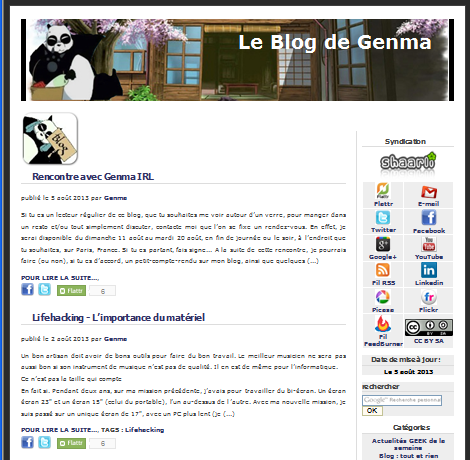
\includegraphics[width=5cm,height=5cm]{./images/blog.png} 
\end{columns}
\end{frame}

%----------------------------------------------------------------------------------------
\begin{frame}
\Huge{\centerline{Introduction}}
\end{frame}

%------------------------------------------------
\begin{frame}
\frametitle{Introduction}

\justifying{
La "protection de sa vie privée et de ses données personnelles" va bien au delà de la compréhension, de l'usage et de la maitrise de logiciels.\\~\\
Je vous propose d'aborder à travers différents thèmes, différentes problématiques, que je soumets à votre réflexion.
\\~\\
Et qui vous montreront quelques points à considérer, à approfondir...
}
\end{frame}

%----------------------------------------------------------------------------------------
\begin{frame}
\Huge{\centerline{Le celebrity gate}}
\end{frame}
%------------------------------------------------

\begin{frame}
\frametitle{Le celebrity gate}
\justifying{Des photos de femmes célèbres nues ont été mises en lignes. Elles avaient été récupérées à partir des comptes ICloud (le Cloud d'Apple).
}
\end{frame}

\begin{frame}
\frametitle{Illustrations}

\justifying{Des photos de nous en soirée peuvent être mise sur les réseaux sociaux}
\begin{center}

\includegraphics[scale=0.4]{./images/Leak01.jpg}
\end{center}
\end{frame}

\begin{frame}
\frametitle{Illustrations}
\justifying{Parfois aves son smarpthone, on prend des photos plus personnelles...}
\begin{center}

\includegraphics[scale=0.5]{./images/Leak02.png}
\end{center}
\end{frame}

\begin{frame}
\frametitle{Illustrations}
\justifying{Voir des photos  \textbf{BEAUCOUP} plus personnelles...}
\begin{center}

\includegraphics[scale=0.5]{./images/Leak03.png}
\end{center}
\end{frame}

\begin{frame}
\frametitle{Illustrations}
\justifying{Même \textbf{TRES TRES} personnelles...}
\begin{center}

\includegraphics[scale=0.6]{./images/Leak05.jpg}
\end{center}
\end{frame}

%------------------------------------------------
\begin{frame}
\frametitle{Leak des photos intimes dans le cloud : quelles sont les leçons à tirer?}
\begin{block}{Quelques leçons préliminaires à en tirer :}
\begin{itemize}
\justifying{
\item Ne croyez pas que ça n’arrive qu’aux autres et uniquement aux stars.
 \item Ne stockez pas vos fichiers sensibles sur le cloud, que ce soit des photos ou des documents d’identité.
 \item Si vous devez stocker un fichier sensible en cloud, chiffrez le localement, sur votre ordinateur, avant de l’envoyer.
 \item Ne sous-estimez pas l’importance du mot de passe. 
 \item Préférez une « phrase de passe », évitez les dates de naissance et les prénoms, essayez d’avoir un mot de passe différent pour chaque compte.
}
\end{itemize}
\end{block}
\end{frame}

%----------------------------------------------------------------------------------------
\begin{frame}
\Huge{\centerline{Les objets connectés}}
\end{frame}
%------------------------------------------------

\begin{frame}
\frametitle{Une carte de géolocalisation des photos de chat 1/2}
\justifying{
Un artiste s'est amusé à récupérer toutes les photos de chats qu'il trouvait sur leweb et en se basant sur les données de géolocalisation de ces photos, à placer celles-ci sur une carte du monde. Voici ce que ça a donné : 
}
\begin{center}
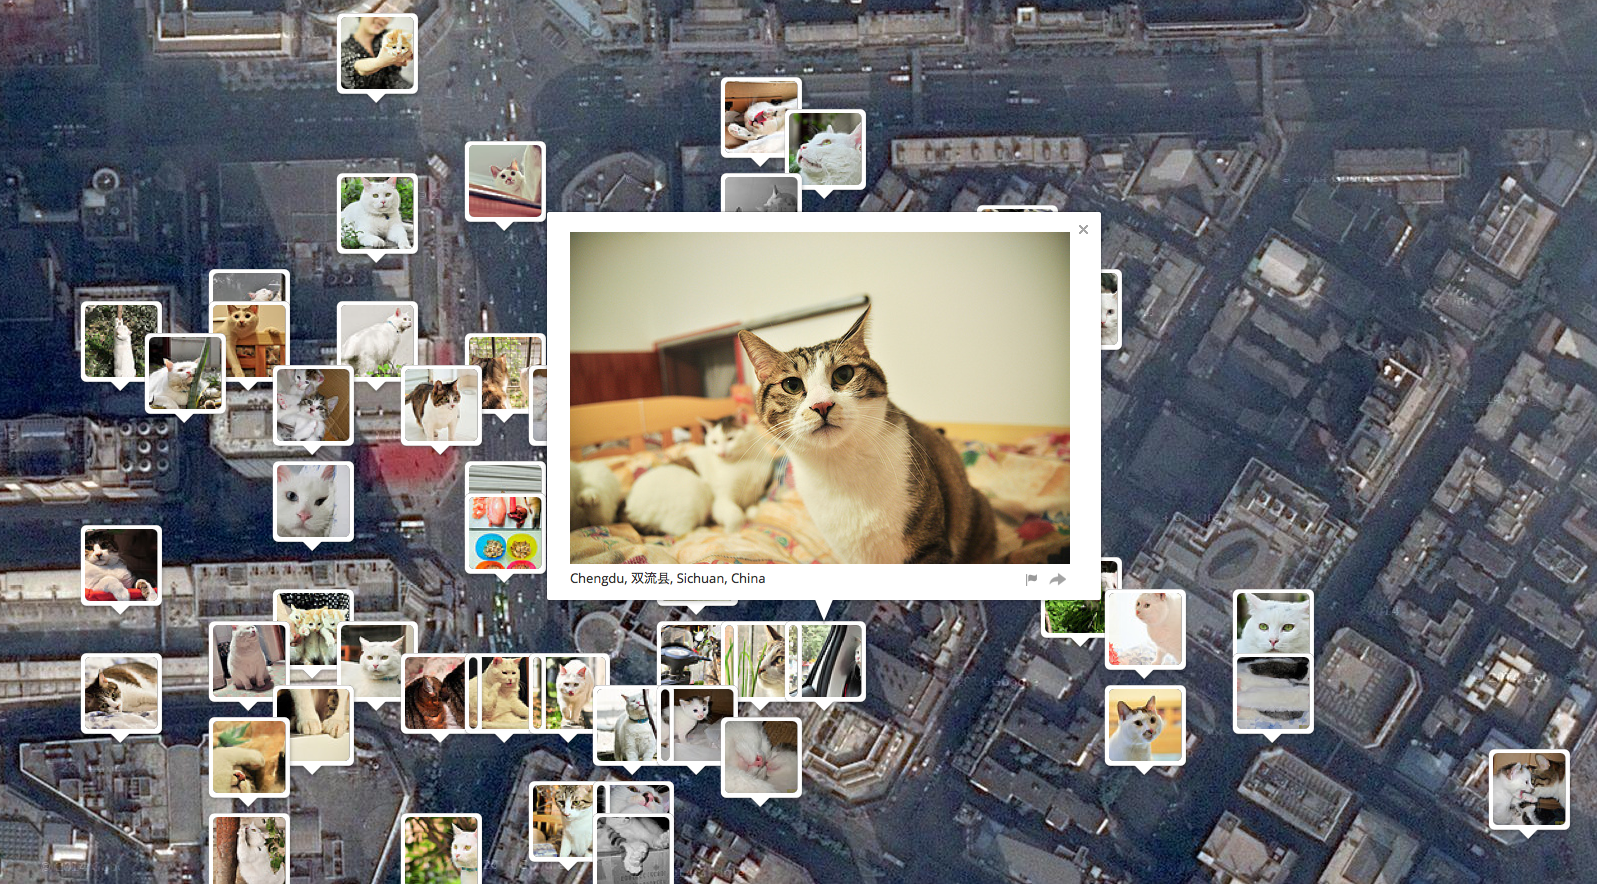
\includegraphics[scale=0.3]{./images/Chat_geolocalisaion.png}
\end{center}
\end{frame}

%------------------------------------------------
\begin{frame}
\frametitle{Une carte de géolocalisation des photos de chat 2/2}
On sait donc quel chat habite où - qui a un chat.
\\~\\
Réfléchissez-y.  \textbf{Et si quelqu'un fasait la même chose mais avec d'autres photos...}
\end{frame}


 %------------------------------------------------
\begin{frame}
\frametitle{Les assurances et les objets connectés}
\justifying{
Les applications pour smartphone tout comme les objets connectés (bracelets)captent votre rythme cardiaque, analysent les photos de vos repas ou comptent le nombre de pas que vous effectuez dans une journée. 
\\~\\
Le but de l'accumulation de toutes ces données afin aux compagnies d’assurances, publicitaires et autres professionnels de la « santé ».
\\~\\
Le risque est de payer plus cher son assurance car on n'a pas ce type d'objet. Donc on acceptera d'être surveillé pour des raisons de baisse de prix....
}
\end{frame}

%------------------------------------------------
\begin{frame}
\frametitle{Des exemples}
\begin{block}{Apple, avec HealthKit}
\begin{itemize}
\justifying{
\item Apple veut les vendre aux assurances pour permettre aux assureurs de conditionner des remboursements ou divers avantages tarifaires à un comportement sanitaire exemplaire, surveillé par la collecte de données en temps réel. 
}
\end{itemize}
\end{block}
\end{frame}

%------------------------------------------------
\begin{frame}
\frametitle{Illustrations}
\begin{center}
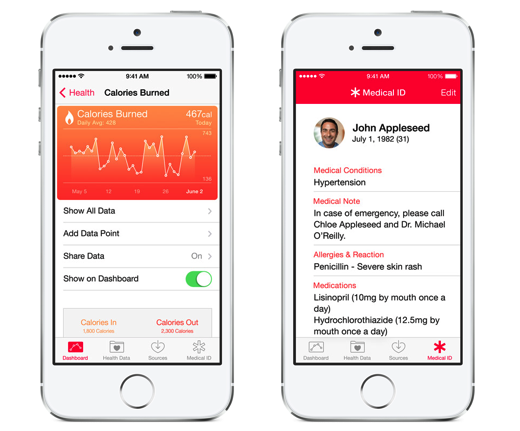
\includegraphics[scale=0.5]{./images/Apple_IOS_DonneesMedicales.png}
\end{center}
\end{frame}

\begin{frame}
\frametitle{Illustrations}
\begin{center}
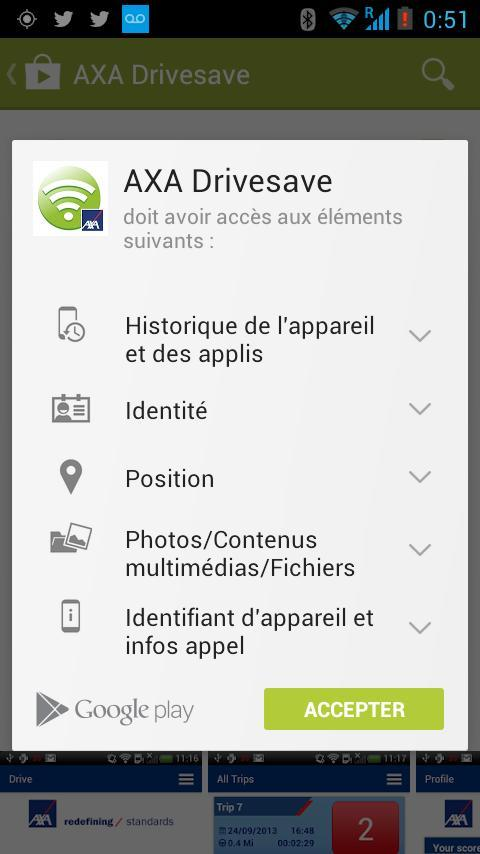
\includegraphics[scale=0.3]{./images/AXA_assurance_gps.jpg} 
\end{center}
\end{frame}

%----------------------------------------------------------------------------------------
\begin{frame}
\Huge{\centerline{Quand on "prête" }}
\Huge{\centerline{sa connexion Internet...}}
\end{frame}
%------------------------------------------------
\begin{frame}
\frametitle{Orange - Connexion Wifi à une livebox}

\begin{block}{Accès au webmail}
\begin{itemize}
\justifying{
\item Lorsque vous êtes connecté à une Livebox, vous êtes implicitement identifié sur orange.fr et pouvez accéder directement à la messagerie Orange. 
\item Il est possible de ne pas être automatiquement identifié sur orange.fr, mais pour cela, il faut avoir créer un compte secondaire.
}
\end{itemize}
\end{block}

\begin{block}{Il n’y pas de réseau “invité” distinct sur la Livebox}
\begin{itemize}
\justifying{
\item CONSEQUENCE : N'importe qui accède au réseau (un ami à qui on donne le code) à donc accès à toute la correspondance mail, aux factures détaillées de téléphone et au moyen de changer tous les mots de passe...
}
\end{itemize}
\end{block}
\end{frame}

\begin{frame}
\frametitle{Freemobile - Partage de connexion}
\begin{block}{Il est possible de partager sa connexion 3G/4G en Wifi (par exemple). }
\begin{itemize}
\justifying{
\item Problème : on est automatiquement authentifié sur le site mobile.free.fr
\item CONSEQUENCE : Toute personne connecté à la connexion partagée a donc accès au compte et peut voir/modifier les options, voir les factures, etc. 
}
\end{itemize}
\end{block}
\begin{center}
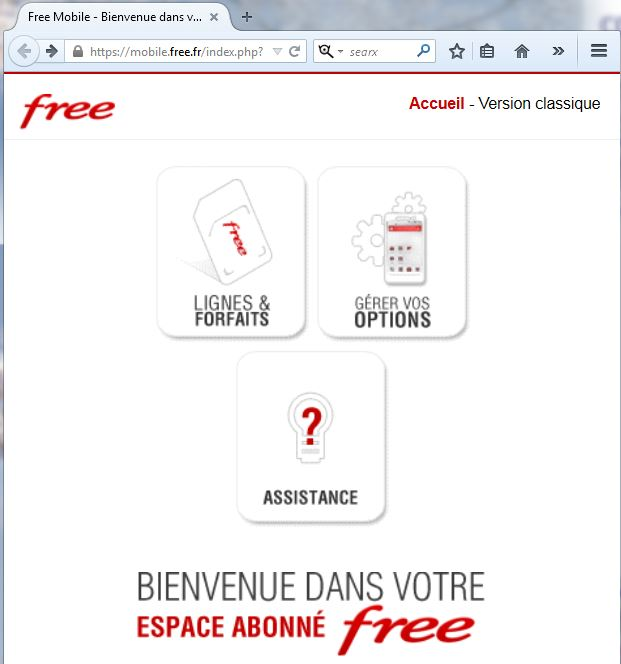
\includegraphics[scale=0.4]{./images/PartageConnexion_Freemobile.jpg}
\end{center}
\end{frame}

%------------------------------------------------
\begin{frame}
\frametitle{Les services Cloud des FAI}
\begin{block}{FAI : Fournisseur d'accès (Bouygues, Orange, SFR...)}
\begin{itemize}
\justifying{
\item  Ces 3 là proposent de "Sauvegardez automatiquement ses photos et autres documents dans leur cloud, un espace totalement privé et confidentiel..."
\item Cela se fait (uniquement) via un logiciel sous Windows, logiciel fermé.
}
\end{itemize}
\end{block}
Quelle confiance accorde-t-on à ces services...
\end{frame}


%----------------------------------------------------------------------------------------
\begin{frame}
\Huge{\centerline{Comment un pseudonymat}}
\Huge{\centerline{peut voler en éclat...}}
\begin{center}

\includegraphics[scale=0.5]{./images/pseudonymat.jpg}
\end{center}
\end{frame}
%------------------------------------------------
\begin{frame}
\frametitle{Comment un pseudonymat peut voler en éclat ?}
\begin{block}{Différents cas d'erreurs}
\begin{itemize}
\justifying{
\item Lors d'une démonstration, avoir un Thunderbird et différents comptes dont un sous la forme prenom.nom
\item Le login du PC sous la forme prénom.nom
}
\end{itemize}
\end{block}

\begin{block}{Cookies, Adresse IP...}
\begin{itemize}
\justifying{
\item Une même IP et des comptes nominatifs et sous pseudonymes (cas de Linkedin)
}
\end{itemize}
\end{block}

\begin{block}{Les réseaux sociaux et ses amis}
\begin{itemize}
\justifying{
\item J'ai mes "vrais" amis associés à mon compte Genma.
}
\end{itemize}
\end{block}

\end{frame}
%------------------------------------------------
\begin{frame}
\frametitle{Wikipedia}
\begin{center}
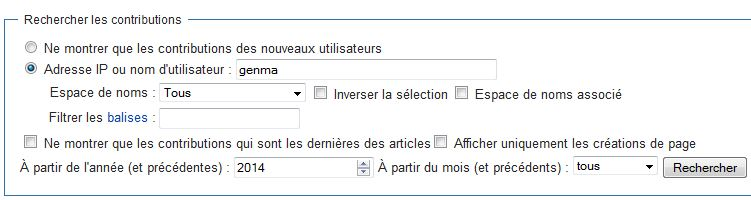
\includegraphics[scale=0.5]{./images/wikipedia_ip.jpg}
\end{center}
\begin{block}{Possibilité de recherche par pseudonyme ou par adresse IP}
\begin{itemize}
\justifying{
\item Si une même personne édite Wikipedia avec un compte sous pseudonyme et un compte nominatif, avec la même adresse IP, on peut faire le lien de façon assez simple.
\item  Si c’est un grand contributeur, on peut avoir toute une liste de ses centres d’intérêts/du type de connaissances qu’elle est susceptible d’avoir de part les thèmes des pages sur lesquelles il y a eu des contributions/modifications...
}
\end{itemize}
\end{block}
\end{frame}

%----------------------------------------------------------------------------------------
\begin{frame}
\Huge{\centerline{Sujets soumis à réflexion}}
\end{frame}
%------------------------------------------------

%------------------------------------------------
\begin{frame}
\frametitle{GoogleFlu et Google trends}
\begin{block}{Présentation de Google Flux sur leur site}
\begin{itemize}
\justifying{
\item Nous avons remarqué que certains termes de recherche étaient des indicateurs efficaces de la propagation de la grippe. Google Flu rassemble donc des données de recherche Google pour fournir une estimation quasiment en temps réel de cette propagation à l'échelle mondiale. \url{http://www.google.org/flutrends/}
\item On peut aussi voir les recherches temps réels, par mot clef, pays... \url{https://www.google.com/trends/}
}
\end{itemize}
\end{block}
\justifying{
Tout cela ne me laisse pas indifférent quand à \textbf{ la puissance de Google}. Et vous?
}
\end{frame}

%------------------------------------------------
\begin{frame}
\frametitle{A méditer}
\begin{block}{Twitt de @goetter}
\justifying{
Avant il fallait expliquer aux gens qu'un blog n'était pas forcément un truc qui se termine par .skyblog.com ...
 \\~\\
Maintenant on en est à leur faire comprendre qu'un site web n'est pas forcément une page Facebook.
}
\end{block}
\end{frame}


%----------------------------------------------------------------------------------------
\begin{frame}
\Huge{\centerline{Annexes}}
\end{frame}
%------------------------------------------------

%------------------------------------------------
\begin{frame}
\frametitle{Comment vérifier rapidement la sécurité d'un site?}
\begin{block}{La check-liste}
\begin{itemize}
\justifying{
\item Le site a-t-il une connexion en https? (SSL). 
\item Y-a-t-il intégration d'éléments extérieurs au site en lui-même?
\item Le site utilise-t-il Google Analytics?
\item Le site utilise-t-il Google Fonts?
\item Le site utilise-t-il des régies publicitaires?
\item Le site utilise-t-il Cloudflare?
\item Le DNS est-il géré par Cloudflare?
\item Le site présente-t-il une politique de confidentialité?
\item Le site utilise-t-il les cookies?
\item Le site utilise-t-il des scripts javascripts?
}
\end{itemize}
\end{block}
\end{frame}

%------------------------------------------------
\begin{frame}
\frametitle{Les sites proposant des messageries chiffrées?}
\begin{block}{La check-liste}
\begin{itemize}
\justifying{
\item Y-a-t-il un chiffrement Javascript côté client?
\item Où se trouvent les clefs publiques/privées?
\item Y-a-t-il des détails sur les algos, la technique etc. et à quel point est-ce détaillé?
}
\end{itemize}
\end{block}
\end{frame}
\end{document}	